%\documentclass[handout]{beamer}
\documentclass{BeamerTemplate}


\newcounter{sauvegardeenumi}
\newcommand{\asuivre}{\setcounter{sauvegardeenumi}{\theenumi}}
\newcommand{\suite}{\setcounter{enumi}{\thesauvegardeenumi}}


%\usepackage[latin1]{inputenc}  %modifies preambule

\title{Statistiques descriptives}
\date{}


\begin{document}

\begin{frame}

\titlepage

\end{frame}

\section{Activité 1}
\begin{frame}[t]{Activité 1}
    Soit les temps de transports suivants:
    $$8, 10, 12, 14, 15, 15,  18, 20, 22, 35, 60 $$

    Calculez :
    \begin{itemize}
        \item la moyenne;
        \item la médiane;
        \item le mode;
        \item le quantile d'ordre 27;
        \item la variance échantillonnale.
    \end{itemize}
\end{frame}

\begin{frame}[t]{Activité 1}
    Soit les temps de transports suivants:
    $$8, 10, 12, 14, 15, 15,  18, 20, 22, 35, 60 $$

    Calculez :
    \begin{itemize}
        \item la moyenne -> 20,82;
        \item la médiane -> 15;
        \item le mode -> 15;
        \item le quantile d'ordre 27 -> 13 ou 12,94;
        \item la variance échantillonnale -> 221,96.
    \end{itemize}
\end{frame}

\section{Activité 2}

\begin{frame}[t]{Activité 2}
\begin{center}
    

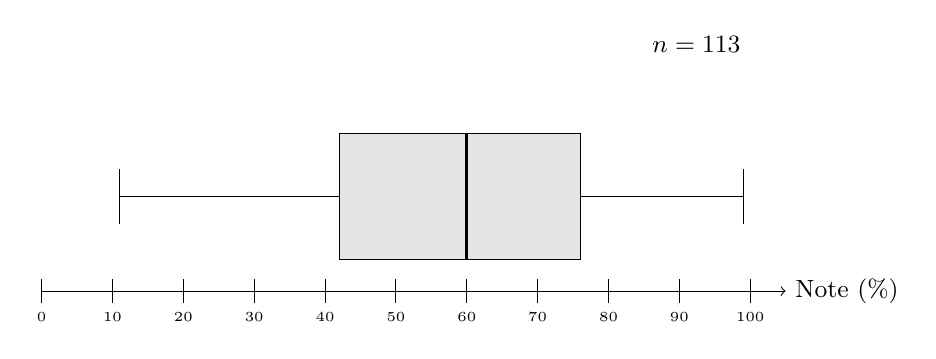
\begin{tikzpicture}[x=0.09cm,y=1cm] % 1 % = 0.09 cm (longueur de l'axe)

% --------- PARAMÈTRES ----------
\def\min{11}      % whisker bas
\def\qone{42}     % Q1
\def\med{60}      % médiane
\def\qthree{76}   % Q3
\def\max{99}      % whisker haut
\def\mean{63}     % moyenne (point noir)
\def\n{113}       % effectif

\def\yaxis{0}     % position verticale de l'axe
\def\ybox{1.2}    % position verticale du centre de la boîte (décale la boîte)
\def\hh{0.8}      % demi-hauteur de la boîte
% --------------------------------

% Axe horizontal 0..100 (sous la boîte)
\draw[->] (0,\yaxis) -- (105,\yaxis) node[right]{\small Note (\%)};
\foreach \p in {0,10,...,100}{
  \draw (\p,\yaxis+0.15) -- (\p,\yaxis-0.15) node[below] {\tiny \p};
}

% Boîte (Q1..Q3) décalée à y=\ybox
\draw[fill=gray!20] (\qone,\ybox-\hh) rectangle (\qthree,\ybox+\hh);

% Médiane
\draw[very thick] (\med,\ybox-\hh) -- (\med,\ybox+\hh);

% Whiskers + chapeaux
\draw (\qone,\ybox) -- (\min,\ybox);
\draw (\qthree,\ybox) -- (\max,\ybox);
\draw (\min,\ybox-0.35) -- (\min,\ybox+0.35);
\draw (\max,\ybox-0.35) -- (\max,\ybox+0.35);




% Effectif en haut à droite
\node[anchor=south east] at (100,\ybox+\hh+0.9) {\small $n=\n$};

\end{tikzpicture}
\end{center}
\end{frame}


\begin{frame}[t]{Activité 2}
\begin{center}
    

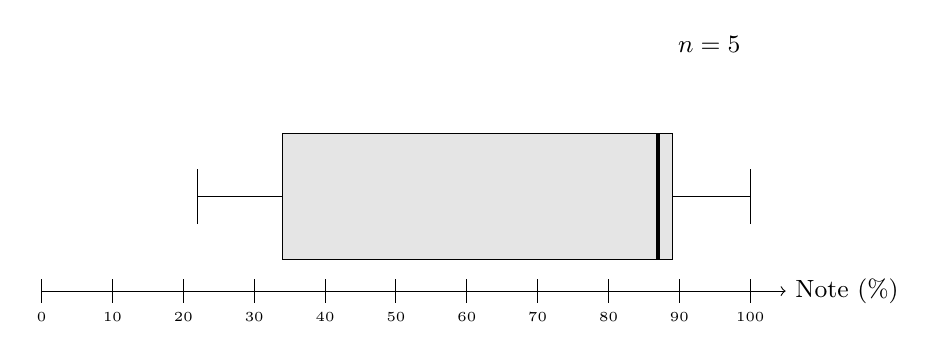
\begin{tikzpicture}[x=0.09cm,y=1cm] % 1 % = 0.09 cm (longueur de l'axe)

% --------- PARAMÈTRES ----------
\def\min{22}      % whisker bas
\def\qone{34}     % Q1
\def\med{87}      % médiane
\def\qthree{89}   % Q3
\def\max{100}      % whisker haut
\def\mean{63}     % moyenne (point noir)
\def\n{5}       % effectif

\def\yaxis{0}     % position verticale de l'axe
\def\ybox{1.2}    % position verticale du centre de la boîte (décale la boîte)
\def\hh{0.8}      % demi-hauteur de la boîte
% --------------------------------

% Axe horizontal 0..100 (sous la boîte)
\draw[->] (0,\yaxis) -- (105,\yaxis) node[right]{\small Note (\%)};
\foreach \p in {0,10,...,100}{
  \draw (\p,\yaxis+0.15) -- (\p,\yaxis-0.15) node[below] {\tiny \p};
}

% Boîte (Q1..Q3) décalée à y=\ybox
\draw[fill=gray!20] (\qone,\ybox-\hh) rectangle (\qthree,\ybox+\hh);

% Médiane
\draw[very thick] (\med,\ybox-\hh) -- (\med,\ybox+\hh);

% Whiskers + chapeaux
\draw (\qone,\ybox) -- (\min,\ybox);
\draw (\qthree,\ybox) -- (\max,\ybox);
\draw (\min,\ybox-0.35) -- (\min,\ybox+0.35);
\draw (\max,\ybox-0.35) -- (\max,\ybox+0.35);




% Effectif en haut à droite
\node[anchor=south east] at (100,\ybox+\hh+0.9) {\small $n=\n$};

\end{tikzpicture}
\end{center}


\end{frame}



\section{Activité 3}


\begin{frame}{Criminalité}
\begin{center}
        \large «La criminalité sur le campus en hausse de 50\%.»\footnote{Statistique inventée.}

        \uncover<2->{\small Dans l'article, on constate que le nombre de crimes est passé de 4 à 6.}
\end{center}

\end{frame}

\begin{frame}{Salaire moyen}
\begin{center}
        \large «Le salaire moyen est passé de 59 000\$ à 61 000\$ au pays cette année.»\footnote{Statistique inventée.}
        
        \uncover<2->{\small Le salaire médian est passé de 41 000\$ à 40 500\$.}
\end{center}

\end{frame}


\begin{frame}{Salaire moyen}
\begin{center}
        \large «Notre supplément offre 200\% de vitamine C!»\footnote{Statistique inventée.}
\end{center}



\end{frame}

\begin{frame}{Salaire moyen}
\begin{center}
        \large «Notre médicament diminue de 75\% la douleur!»\footnote{Statistique inventée.}
\end{center}



\end{frame}

\end{document}


